\documentclass[10pt,a4paper]{ctexart}
\usepackage[margin=2cm]{geometry}
\usepackage{graphicx}
\usepackage{hyperref}
\usepackage{amsmath}    % 提供方程环境
\usepackage{physics}    % 简化向量、微分算子语法
\newcommand{\myspace}[1]{\par\vspace{#1\baselineskip}} %自定义空一行
\usepackage{fancyhdr}
\usepackage{wrapfig}
\usepackage{booktabs} % 添加 booktabs 宏包
\usepackage{array}
\usepackage{float}
\usepackage{makecell}
\pagestyle{fancy}
\fancyhf{}  % 清除所有页眉页脚
\fancyfoot[C]{\thepage}  % 在页脚中央设置页码
\renewcommand{\headrulewidth}{0pt}  % 去掉页眉横线
\renewcommand{\footrulewidth}{0pt}  % 去掉页脚横线

\usepackage{hyperref}
\hypersetup{
    colorlinks=true,
    linkcolor=blue,
    filecolor=magenta,      
    urlcolor=cyan,
    pdftitle={Overleaf Example},
    pdfpagemode=FullScreen,
    }

\usepackage{titlesec}

% 重新定义section格式
\titleformat{\section}
  {\normalfont\Large\bfseries}
  {\chinese{section}、}
  {0pt}
  {}

% 给出常用字号的自定义指令
\newcommand{\chuhao}{\fontsize{42pt}{48pt}\selectfont}
\newcommand{\xiaochu}{\fontsize{36pt}{42pt}\selectfont}
\newcommand{\xiaoer}{\fontsize{18pt}{21.6pt}\selectfont}
\newcommand{\sanhao}{\fontsize{16pt}{20pt}\selectfont}
\newcommand{\xiaosan}{\fontsize{15pt}{18pt}\selectfont}
\newcommand{\sihao}{\fontsize{14pt}{18pt}\selectfont}
\newcommand{\xiaosi}{\fontsize{12pt}{16pt}\selectfont}
\newcommand{\wuhao}{\fontsize{10.5pt}{12.6pt}\selectfont}

% 定义中文数字转换
\titleformat{\section}
  {\normalfont\Large\bfseries}
  {\zhnum{section}、}  % 使用\zhnum而不是\chinese
  {0pt}
  {}

% 标题设置
\title{\xiaochu\textbf{物理实验报告}}
\author{}
\date{}

\begin{document}

\vspace*{36pt} % 顶部空白

% 居中填写区域
\begin{center}
    
\includegraphics[width = 9cm]{figures/head.png}
    
    \xiaochu\textbf{物理实验报告}
    % 预留空白区域
    \vspace{13pt}
    \vspace{13pt}
    \vspace{13pt}
    \vspace{13pt}
    
    \sanhao\textbf{实验名称：\underline{\makebox[10cm]{ 交流电路功率因数实验、组装整流器 }}} \\[10pt]
    \sanhao\textbf{实验桌号：\underline{\makebox[8cm]{  }}} \\[10pt]
    \sanhao\textbf{指导教师：\underline{\makebox[8cm]{  }}} \\[20pt]
    
    % 预留空白区域
    \myspace{7}
    
   \sihao\textbf{班级：\underline{\makebox[6cm]{cc98}}} \\[10pt]
    \sihao\textbf{姓名：\underline{\makebox[6cm]{Hydrofoil}}} \\[10pt]
    \sihao\textbf{学号：\underline{\makebox[6cm]{324010}}} \\[30pt]
    
   \sihao\textbf{实验日期: \underline{\makebox[0.8cm] 2025 }年 \underline{\makebox[0.4cm]12}月\underline{\makebox[0.4cm]18}日  星期\underline{\makebox[0.6cm]四}下午}
    
    \vspace{18pt}
    \sihao 浙江大学物理实验教学中心
    
\end{center}

\newpage

\section{预习报告}

    \subsection{实验综述}
    
    \xiaosi （自述实验现象、实验原理和实验方法，不超过500字，5分）
    
    \myspace{0}
    
    \subsubsection*{日光灯电路与功率因数的提高：}

    日光灯是一种典型的电感性负载电路，它主要由灯管$L$、镇流器$M$、启辉器$S$组成，如图所示。

    \begin{figure}[H]
    \centering
    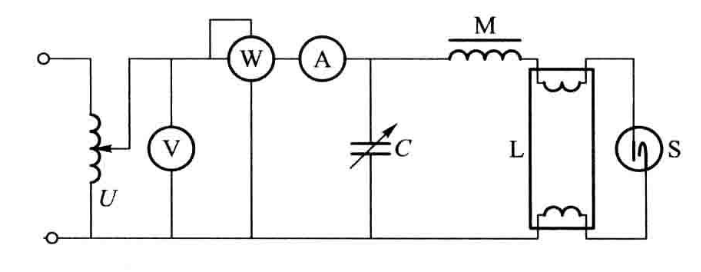
\includegraphics[width=10cm]{figures/日光灯.png}
    \caption{日光灯电路工作原理图}
    \label{fig:图1}
    \end{figure}  

    日光灯通电后，启辉器辉光放电接通电路，电流加热灯丝使其发射电子并气化管内液汞。随后启辉器自动断开，导致串联的镇流器产生瞬间高压，击穿灯管内的汞蒸气形成弧光放电。放电时高速电子撞击汞原子辐射出紫外线，紫外线激发管壁荧光粉吸收能量并发出可见光。灯管点亮后，镇流器利用感抗限制电流，维持其稳定发光。
    
    交流电路中的负载分为阻性负载、容性负载、感性负载。阻性负载电流和电压相位相同，容性负载电流超前电压$90^{\circ}$，感性负载电流落后电压$90^{\circ}$。
    
    如果用 $I_L$ 作为相位的参考方向，下图是它们之间的相位矢量图，由图可见 $I_L$ 与 $U_R$ 同相。而纯电感 $L $上的电压 $U_L$ 比 $I_L$ 超前 $\pi/2$，合成的 $U $是总电压的幅值，$\varphi $是 $I_L$ 落后$U$ 的相位角。
    
    \begin{figure}[H]
    \centering
    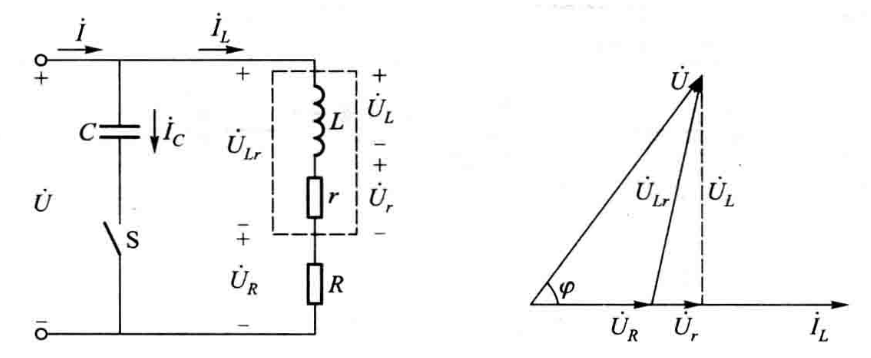
\includegraphics[width=10cm]{figures/相位.png}
    \caption{相位关系}
    \label{fig:图2}
    \end{figure}

    \
    

    \begin{wrapfigure}{r}{0.4\textwidth}
    \centering
    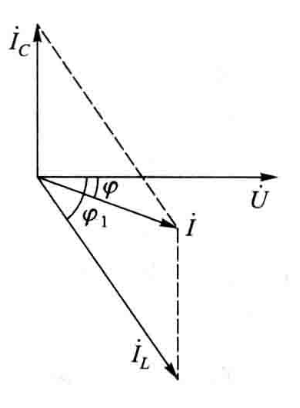
\includegraphics[width=3cm]{figures/并联.png}
    \caption{功率因数的放大}
    \label{fig:图1}
    \end{wrapfigure}

    \

对应提高电感性电路的功率因数，常用的方法就是在靠近感性负载端并联电容器，其电路图如左图所示，由相量图可知原感性负载电流滞后于电压$ \varphi $当并联电容以后
，只要电容的大小选择得当，就可以使并联电容以后的总电流小于原来电感中的电流，使$ \varphi' < \varphi $使功率因数得到提高。  

    \subsubsection*{各种电压的定义及波形因素}
    
    峰峰电压\(V_{PP}\)：表示正弦波峰到波峰之间的电压幅度；
    
    峰值电压\(V_{P}\)：表示正向脉动电压从零电平到最高电压之间的幅度；
    
    平均值电压：\(\bar{V}=\frac{1}{T} \int_{0}^{T} u(t) dt\)；
    
    有效值电压：\(\dot{V}=\sqrt{\frac{1}{T} \int_{0}^{T} u^{2}(t) dt}\)。
    
    \subsubsection*{各波形间的相互关系}
    
    波形系数：\(K_{F}=\frac{\dot{V}}{\bar{V}}\)；波峰系数：\(K_{P}=\frac{V_{P}}{\dot{V}}\)；
    
    由上述两式可得：\(\bar{V}=\frac{V_{P}}{K_{F} \cdot K_{P}}\)。
    
    \begin{wrapfigure}{r}{0.4\textwidth}
    \centering
    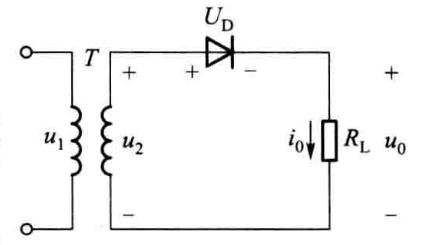
\includegraphics[width=6cm]{figures/半波.png}
    \caption{半波整流电路}
    \label{fig:图1}
    \end{wrapfigure}
    
    
    \subsubsection*{整流电路的类型及特点}

    
    \textbf{1.半波整流}
    
    二极管的反向耐压：电阻负载时承受的反向最大电压为\(\sqrt{2}V_{2}\)；电容负载时承受的反向最大电压为\(2\sqrt{2}V_{2}\)。
    
    输入输出电压关系：输入\(u=\sqrt{2}V_{2}\sin\omega t\)，在二极管导通时忽略电路损耗与门限电压，则：
    
    \(\overline{V_{0}}=\frac{1}{2\pi} \int_{0}^{\pi} u_{2} d(\omega t)=\frac{\sqrt{2}}{\pi}V_{2}≈0.45V_{2}\)。
    
    \begin{wrapfigure}{r}{0.4\textwidth}
    \centering
    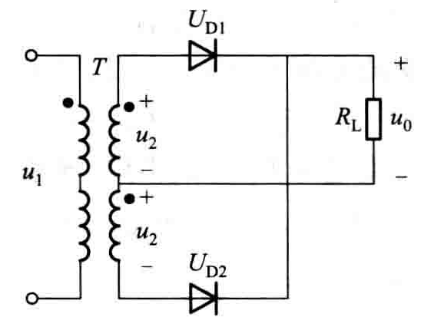
\includegraphics[width=5cm]{figures/全波.png}
    \caption{全波整流电路}
    \label{fig:图1}
    \end{wrapfigure}
    
    \textbf{2.全波整流}
    
    滤波效果及二极管承受反向最大压降与半波整流相同。
    
    优点：利用了电源的正、负周期，电源脉动大大减小。缺点：需要两个整流二极管，变压器需中心抽头，结构相对复杂。
    
    \textbf{3.桥式整流}
    
    滤波效果与前两者相同。二极管承受的最大反向压降由两只二极管共同分担。

    \begin{figure}[H]
    \centering
    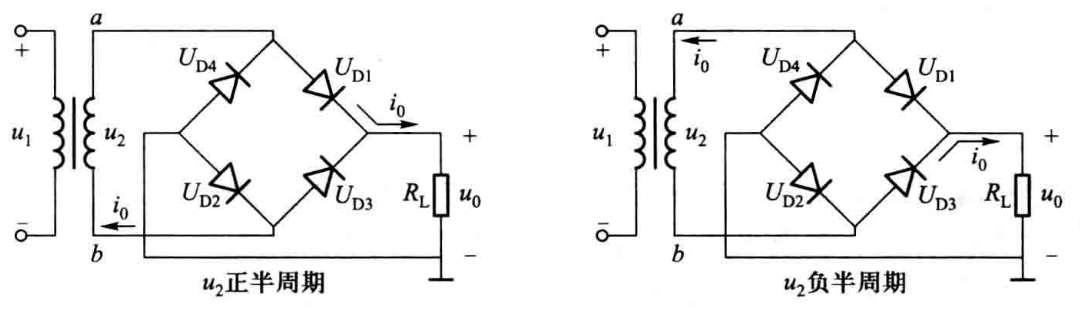
\includegraphics[width=10cm]{figures/桥式.png}
    \caption{桥式整流电路}
    \label{fig:图2}
    \end{figure}

    
    \subsubsection*{滤波电路}
    
    滤波原理（以 RC 为例）：当u为正半周期时，二极管导通，对电容充电，因二极管导通时内阻很小，电容很快被充到峰值。当负半周期时，二极管截止，电容放电，时间常数\(\tau = RC\)。当\(\tau \gg T\)时，电容上电压刚释放一小部分，下一周期二极管又导通，电容充电，如此即可保持输出电压稳定。



    \subsection{实验重点}
    
    \xiaosi（简述本实验的学习重点，不超过100字，3分）

    \begin{enumerate}
        \item 理解功率因数的物理意义；
        \item 掌握提高感性电路功率因数的方法；
        \item 主席日光灯的工作原理，掌握测量日光灯功率的方法；
        \item 根据实验室提供的元件，完成各种整流电路的设计；
        \item 熟悉电子示波器的使用，了解一些常用电子元件的使用方法；
        \item 了解整流器作用，以及整流电路和滤波电路的功能。
    \end{enumerate}
    
    \subsection{实验难点}
    
    \xiaosi（简述本实验的实现难点，不超过100字，2分）

    \begin{enumerate}
        \item 电路搭建精度要求高：半波、全波、桥式整流电路的接线逻辑不同（如全波需变压器中心抽头、桥式需四只二极管合理排布），且元件（二极管、电容、电阻）极性和连接位置易出错，影响电路导通与整流效果。
        \item 仪器操作与波形观测难度：需熟练掌握示波器的连接方式、参数调节（如峰峰值、有效值测量），且滤波前后波形变化细微，需精准区分并记录，读数存在天然浮动误差。
        \item 反向耐压与电路安全控制：二极管反向耐压值需匹配电路电压（如半波整流电容负载时反向电压达\(2\sqrt{2}V_{2}\)），且变压器禁止短路，操作中需规避过载、接线错误等安全风险。
        \item 误差控制与数据分析：实际元件非理想特性（如二极管反向漏电流、元件内阻）、输入电压波动等因素易导致实验数据与理论值偏差，需准确识别误差来源并合理分析。
    \end{enumerate}

\newpage

\section{原始数据}

    \xiaosi （将有老师签名的“自备数据记录草稿纸”的扫描或手机拍摄图粘贴在下方，20分）

    \begin{figure}[htbp]
        \centering
        
\includegraphics[width=14cm]{figures/实验数据.jpg}
        \caption{实验数据}
        \label{fig:图3}
    \end{figure}

\newpage

\section{结果与分析}

    \subsection{数据处理与结果}
    \xiaosi （列出数据表格、选择数据处理方法、给定测量或计算结果，30分）

    \subsubsection{交流功率因数实验}

    根据实验测得数据计算外接不同电容时的功率因数，得到下表：

    \begin{table}[htbp]
    \centering
    \caption{并联电容对电路参数及功率因数的影响}
    \label{tab:power_factor}
    % 使用 resizebox 自动缩放表格以适应页面宽度
    \resizebox{\textwidth}{!}{%
        \begin{tabular}{lcccccccccc}
            \toprule
            $C$ ($\mu$F) & 0 & 9 & 8 & 7 & 6 & 5 & 4 & 3 & 2 & 1 \\
            \midrule
            $P$ (W)    & 24.6  & 26.1  & 24.2  & 26.6  & 24.3  & 24.4  & 24.4  & 24.3  & 24.3  & 27.1 \\
            $U$ (V)    & 225.3 & 225.9 & 225.3 & 225.3 & 225.5 & 225.2 & 224.6 & 225.1 & 224.7 & 225.3 \\
            $I$ (mA)   & 316.0 & 304.5 & 242.1 & 196.1 & 146.6 & 124.0 & 138.4 & 165.5 & 219.1 & 256.8 \\
            \midrule
            % 计算公式：P / (U * I/1000)
            $\lambda= \frac{P}{UI}$ & 0.346 & 0.379 & 0.444 & 0.602 & 0.735 & 0.874 & 0.785 & 0.652 & 0.494 & 0.468 \\
            \bottomrule
        \end{tabular}%
    }
\end{table}

根据上表拟合功率因数与电容大小关系，得到如下曲线：

        \begin{figure}[H]
    \centering
    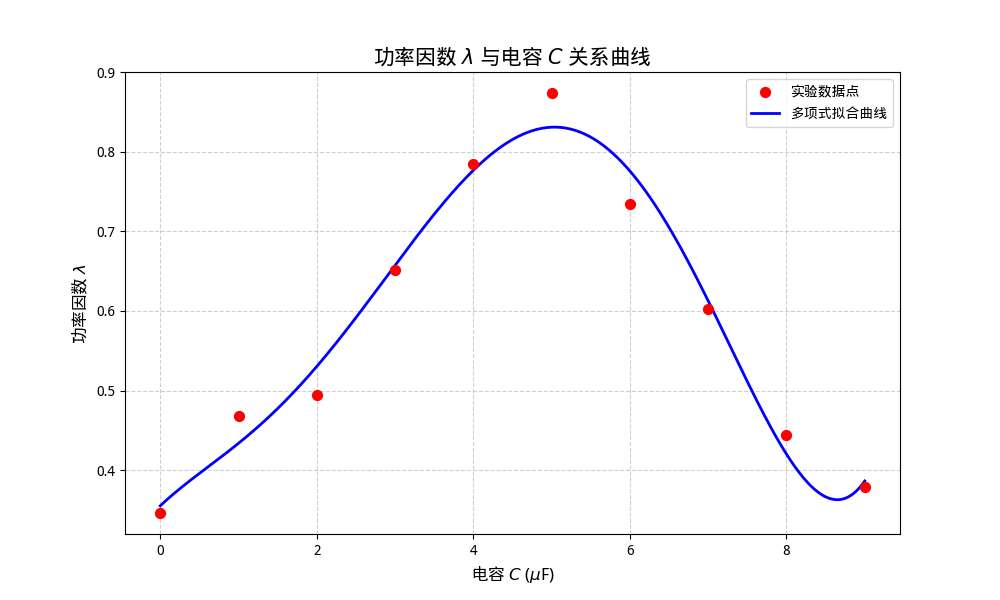
\includegraphics[width=12cm]{figures/Figure_1.png}
    \caption{相位关系}
    \label{fig:图2}
    \end{figure}

    可以得到当$c = 5\mu F$时功率因数达到最大，为$0.874$。

    \subsubsection{组装整流器}
    
    对于不同的整流电路，分别作出整流电路如下：

\begin{table}[H]
    \centering
    \caption{半波整流电路}
    \vspace{0.2cm}
    % 定义6列，全部居中，带竖线
    \begin{tabular}{|c|c|c|c|c|c|}
        \hline
        % 第一行表头：合并单元格
        \multicolumn{2}{|c|}{输入信号} & 
        \multicolumn{3}{c|}{无滤波器输出信号} & 
        \makecell[c]{几十$\mu$F滤波器\\输出信号} \\
        \hline
        % 第二行表头：具体参数
        波形图 & 有效值电压 $U_2$ & 波形图 & 平均值电压 & 有效值电压 & 波形图 \\
        \hline
        % 数据行 1 (使用 vspace 增加高度，模拟空白填空区)
        \rule{0pt}{30pt} 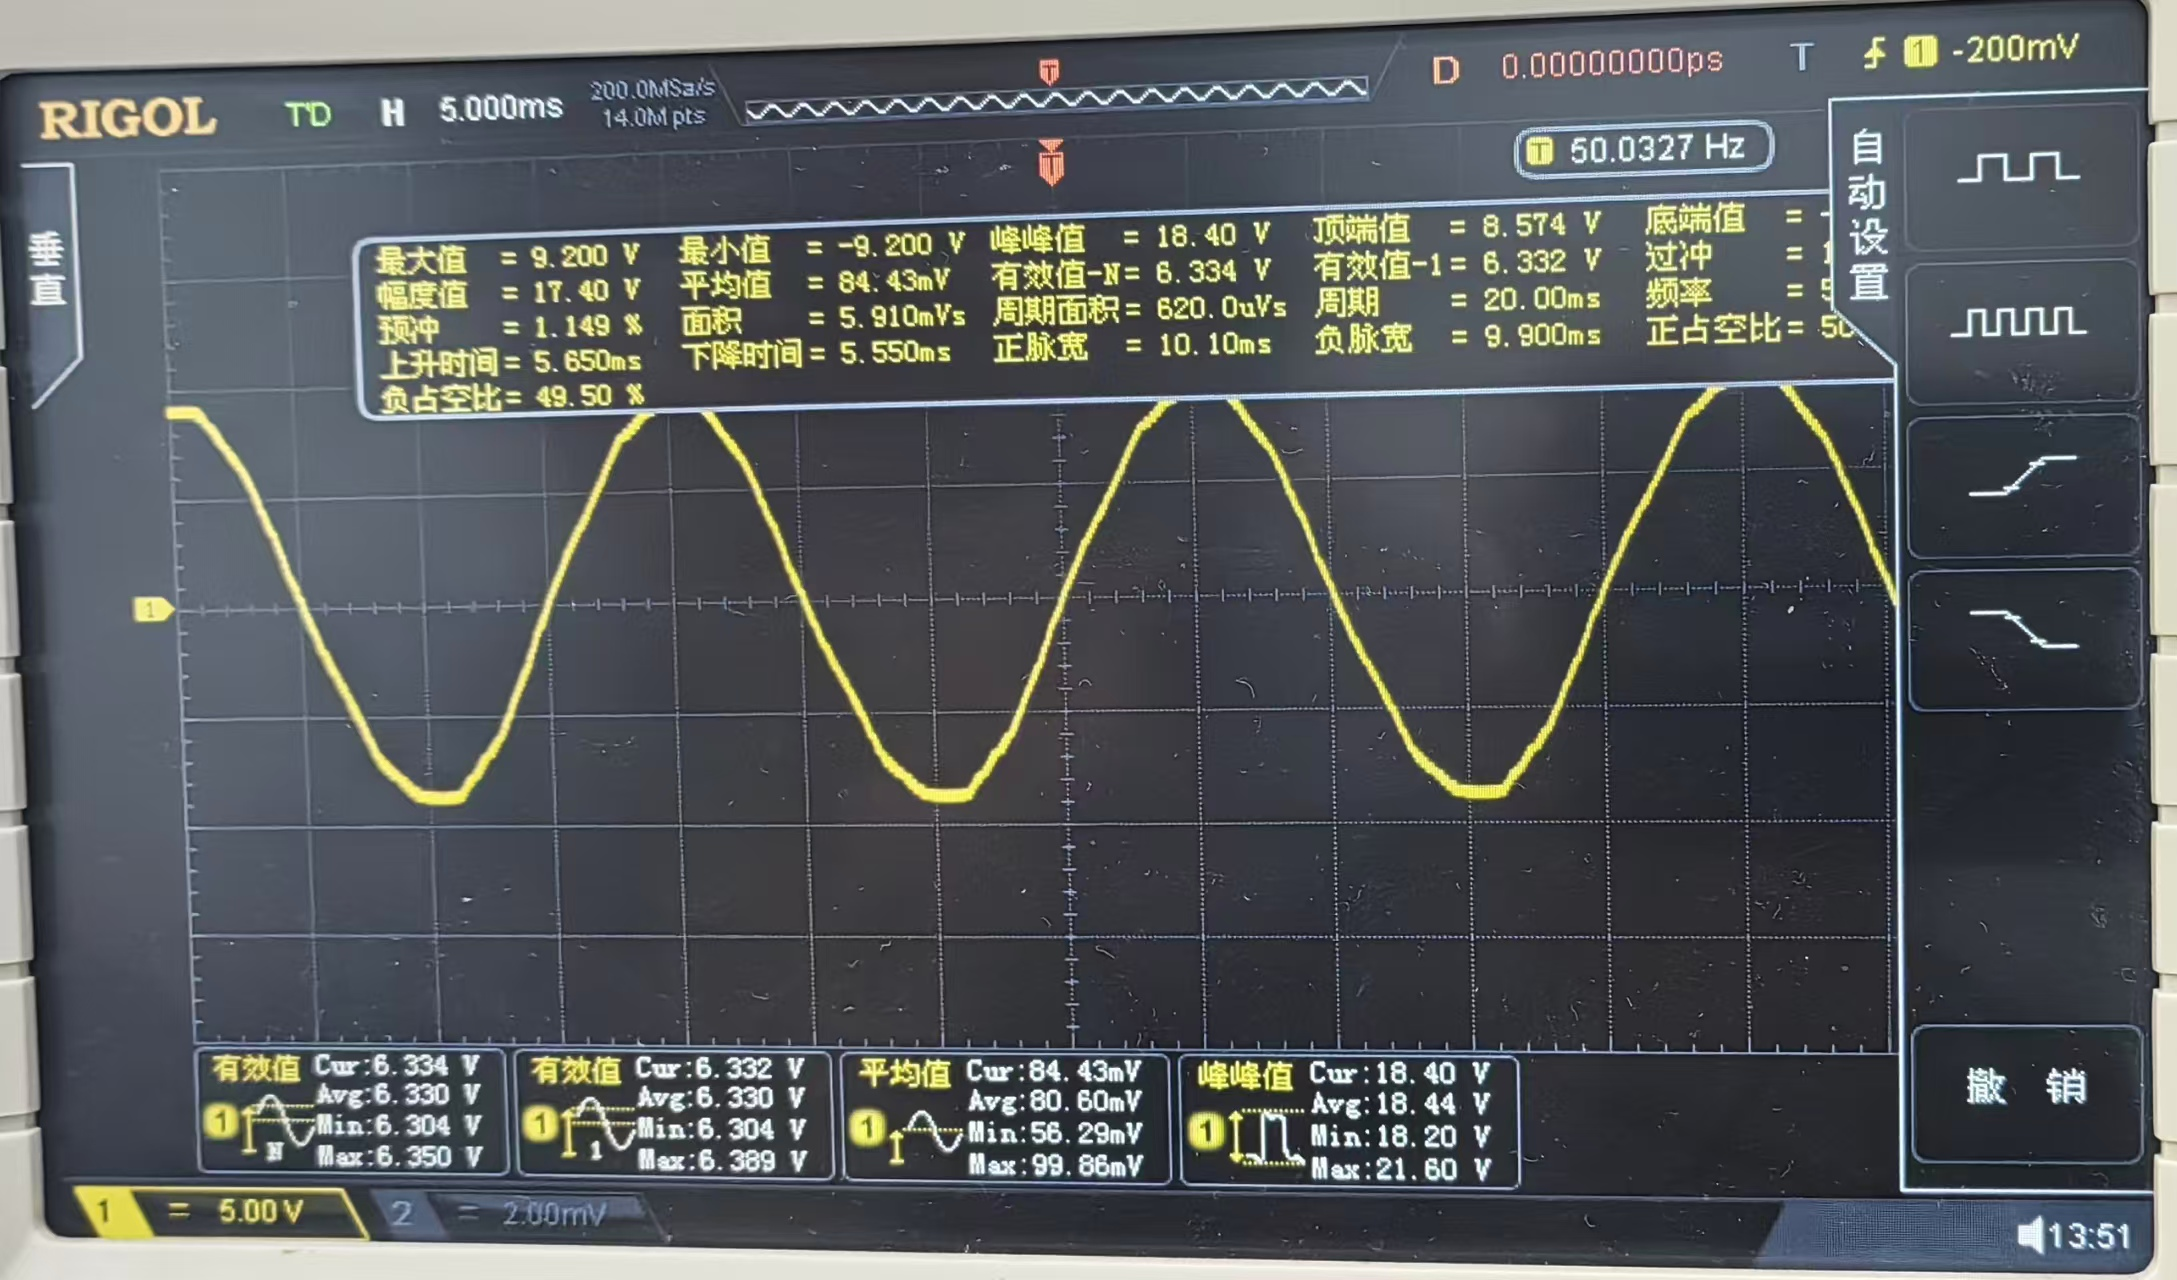
\includegraphics[width=3cm]{figures/1.jpg}& 6.33V&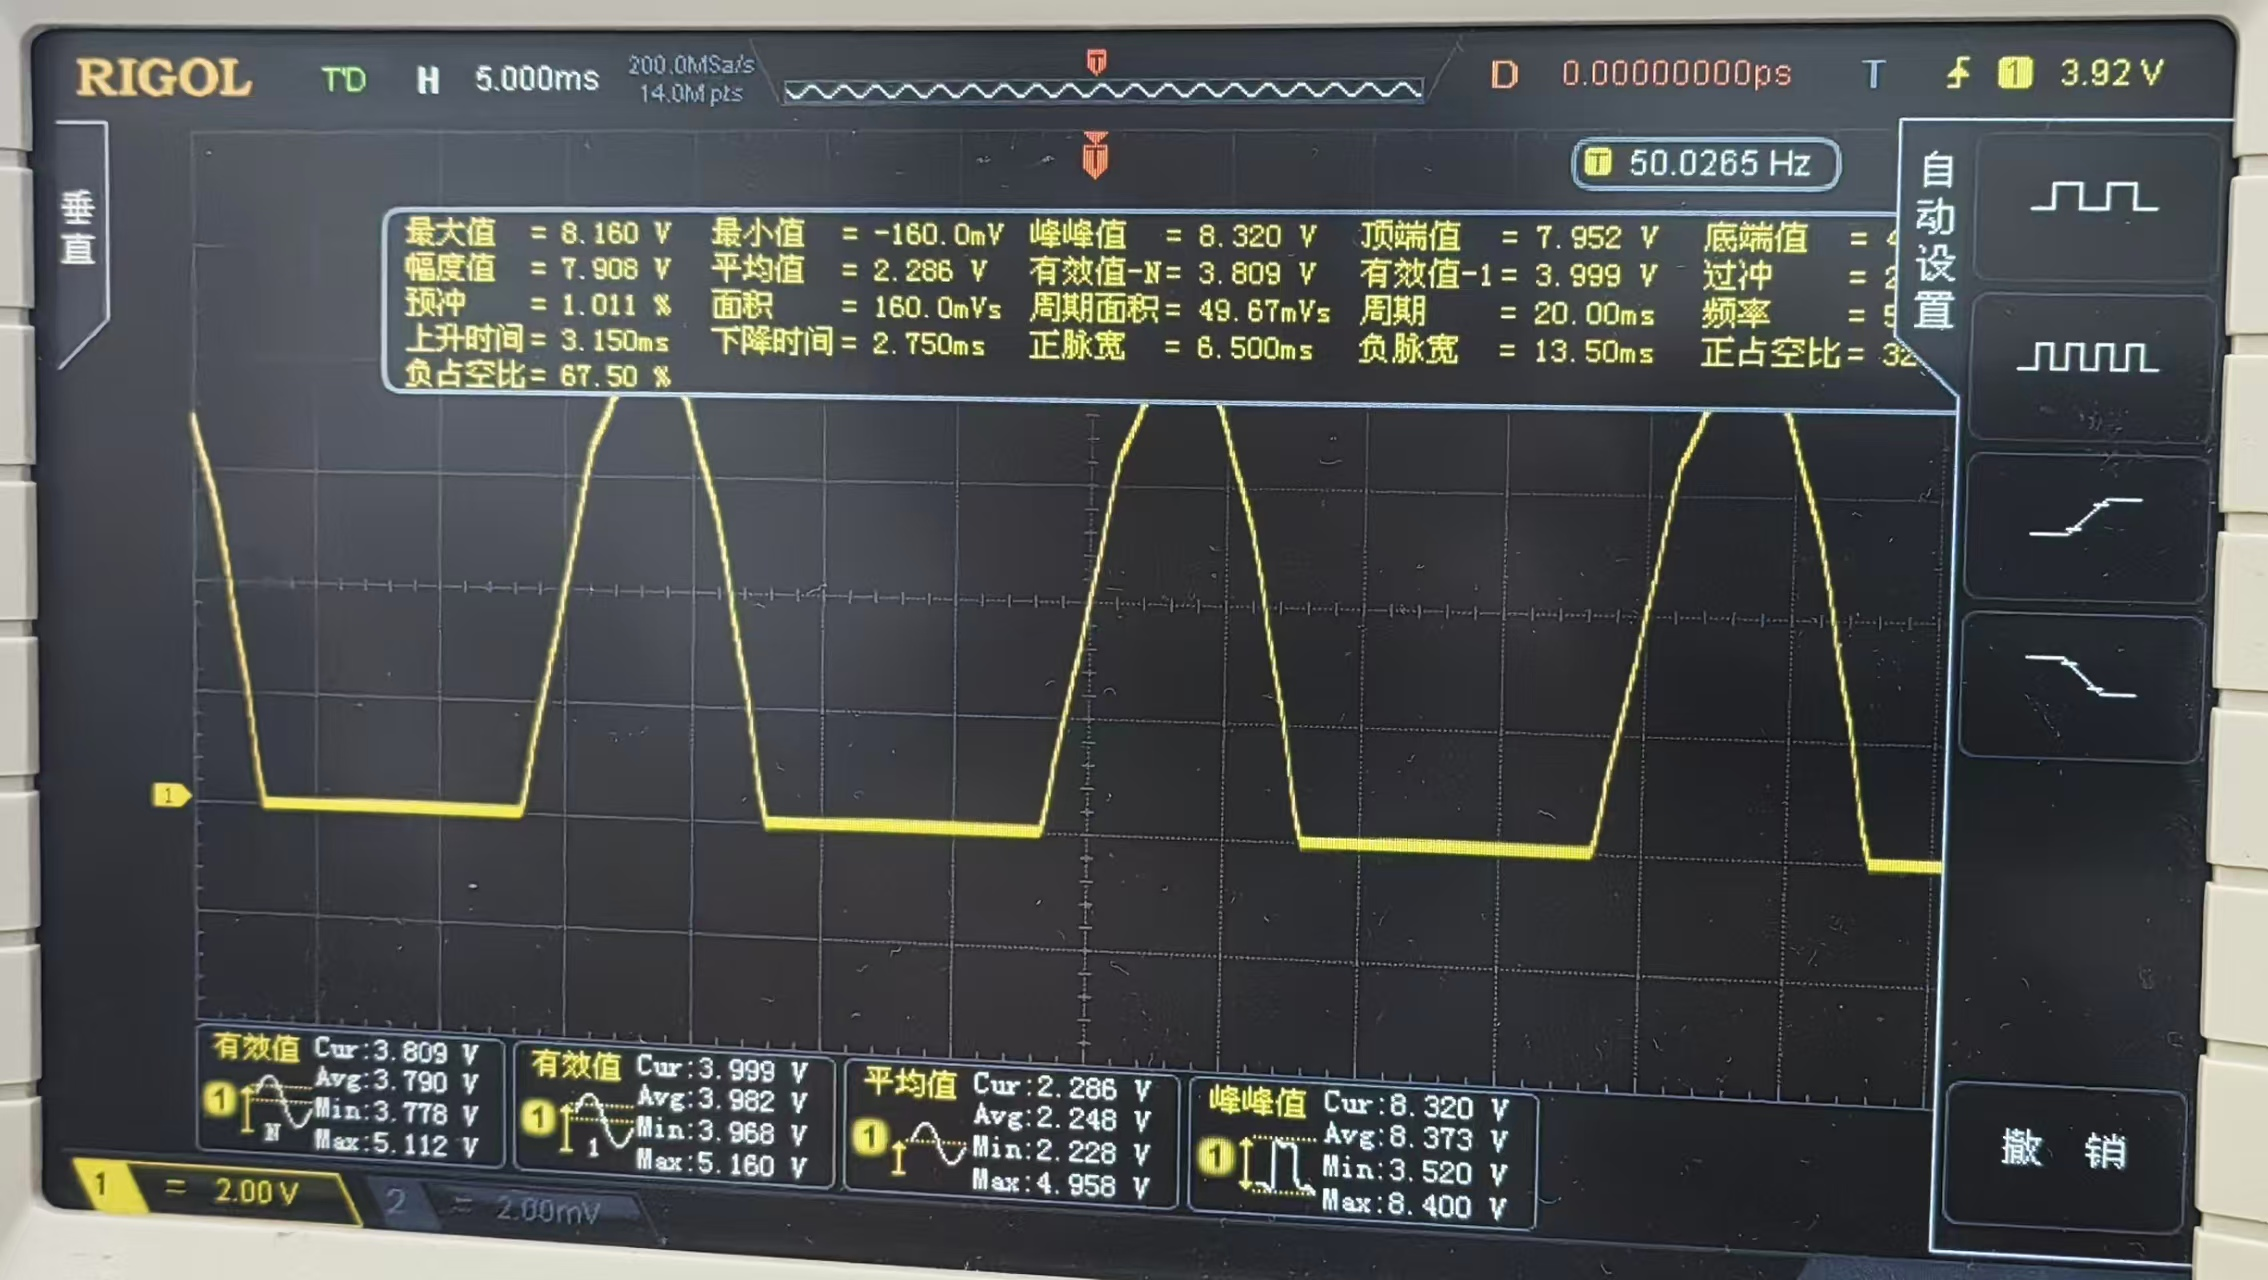
\includegraphics[width=3cm]{figures/2.jpg} &2.29V & 3.99V& 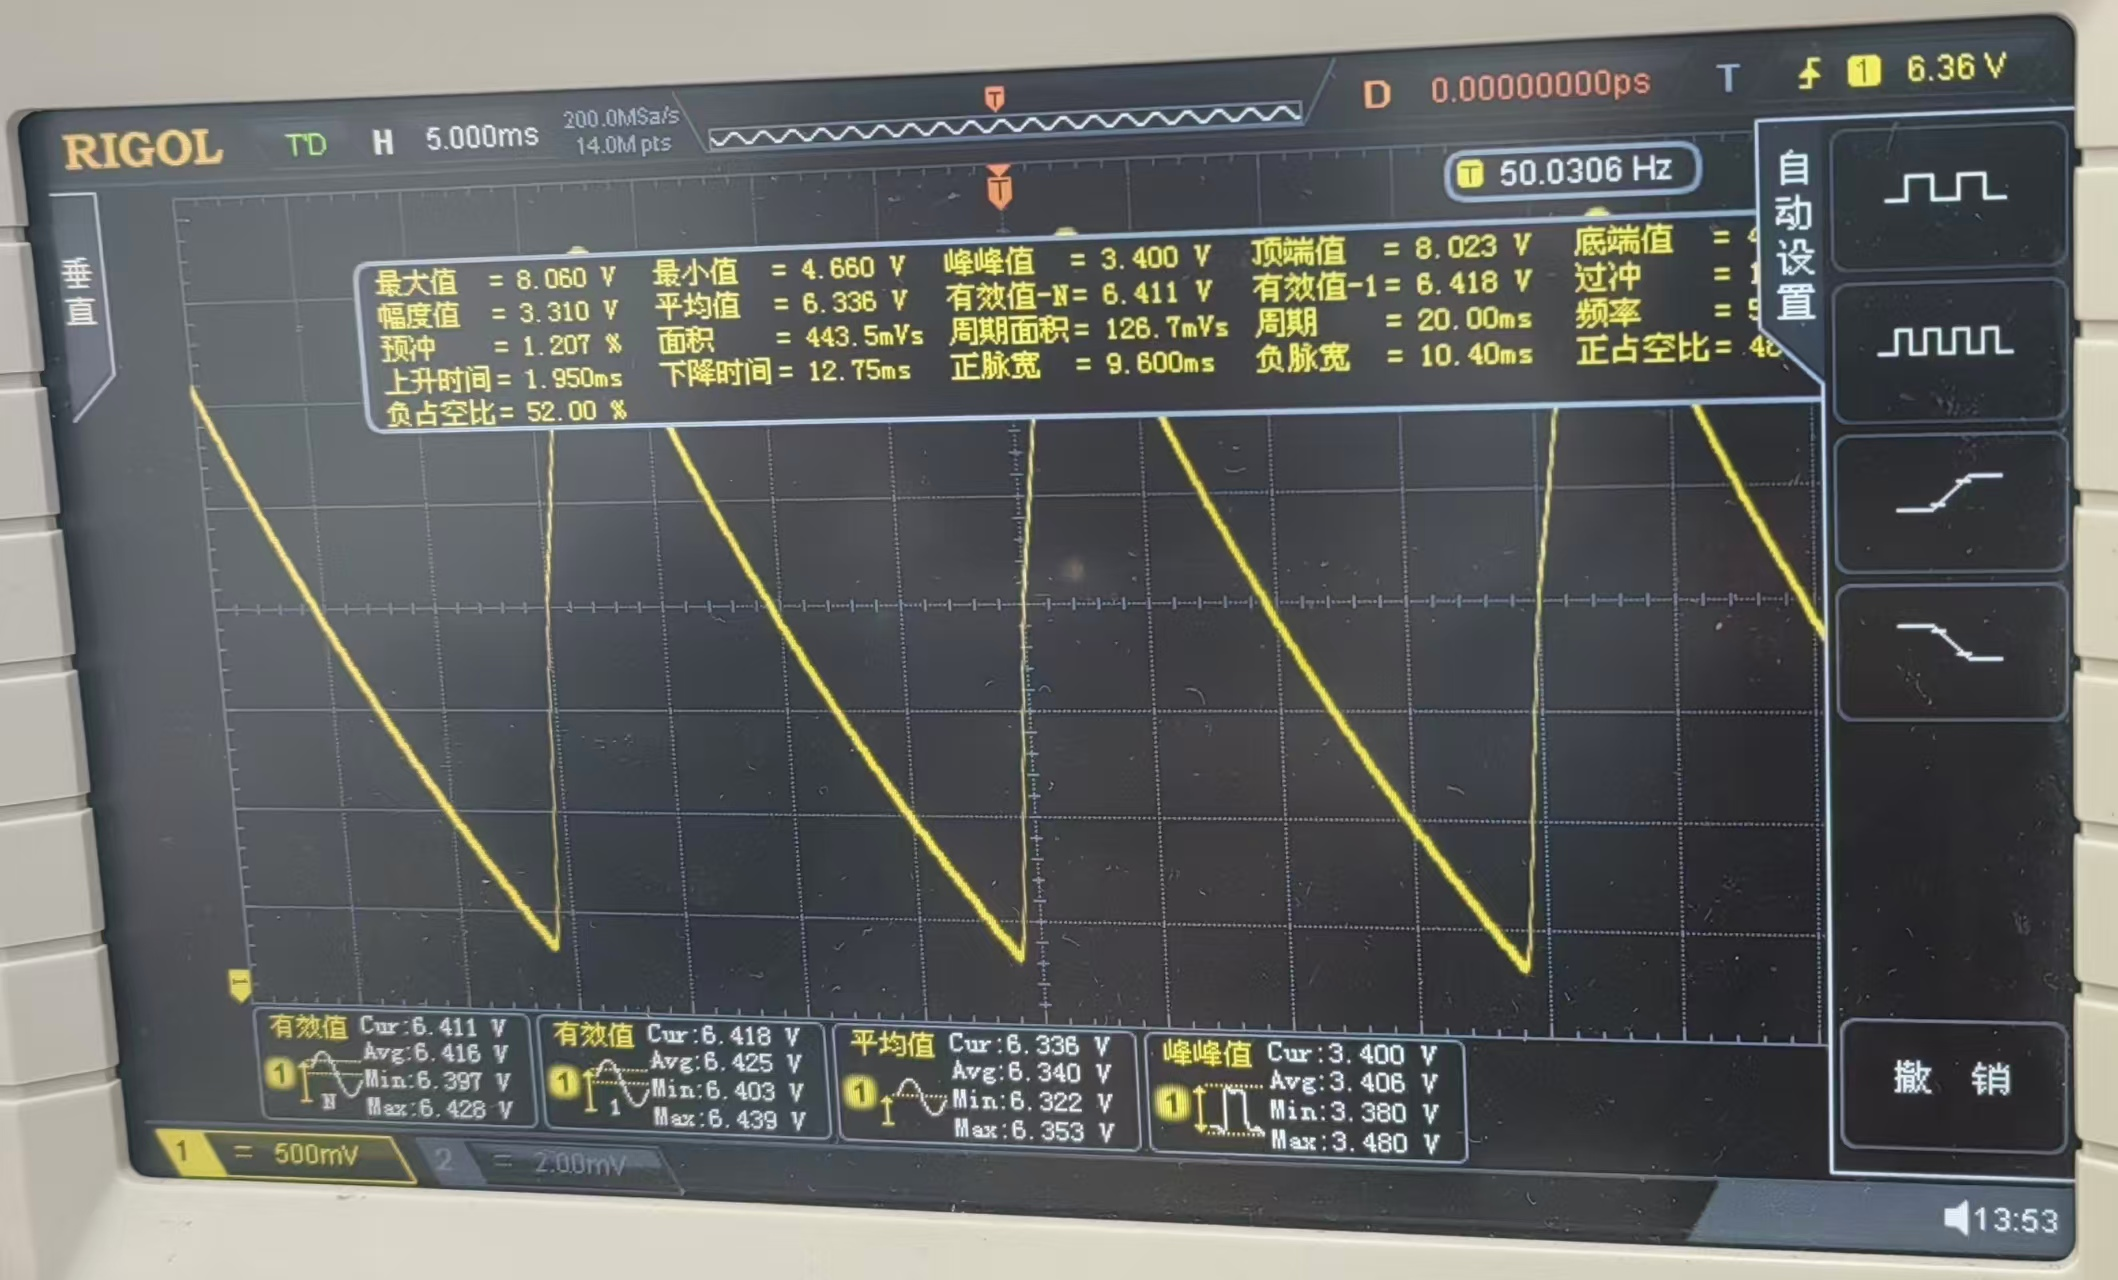
\includegraphics[width=3cm]{figures/3.jpg}\\ 
        \hline
    \end{tabular}
\end{table}

\begin{table}[H]
    \centering
    \caption{全波整流电路}
    \vspace{0.2cm}
    % 定义6列，全部居中，带竖线
    \begin{tabular}{|c|c|c|c|c|c|}
        \hline
        % 第一行表头：合并单元格
        \multicolumn{2}{|c|}{输入信号} & 
        \multicolumn{3}{c|}{无滤波器输出信号} & 
        \makecell[c]{几十$\mu$F滤波器\\输出信号} \\
        \hline
        % 第二行表头：具体参数
        波形图 & 有效值电压 $U_2$ & 波形图 & 平均值电压 & 有效值电压 & 波形图 \\
        \hline
        % 数据行 1 (使用 vspace 增加高度，模拟空白填空区)
        \rule{0pt}{30pt} 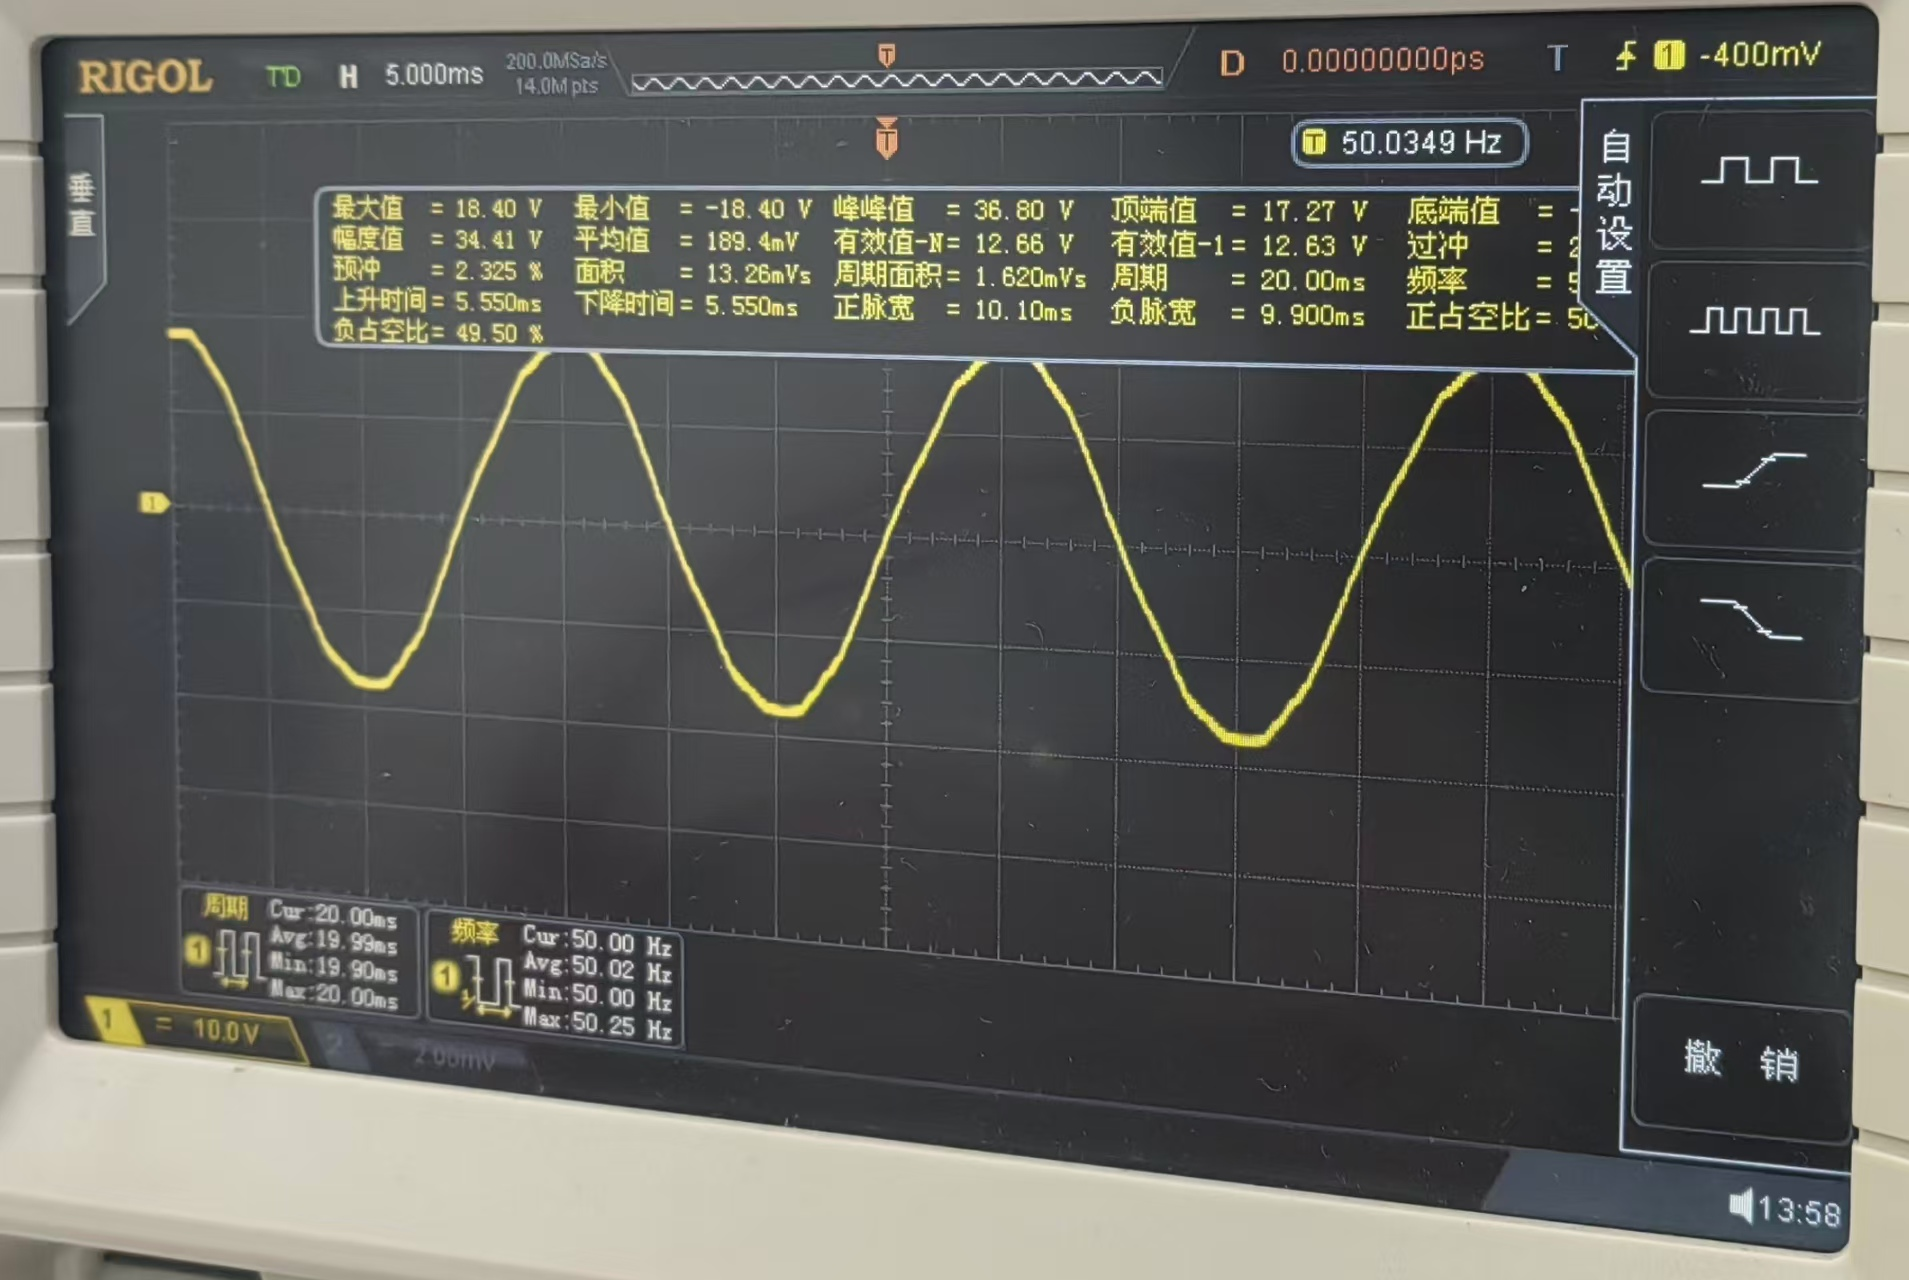
\includegraphics[width=3cm]{figures/4.jpg}& 12.66V&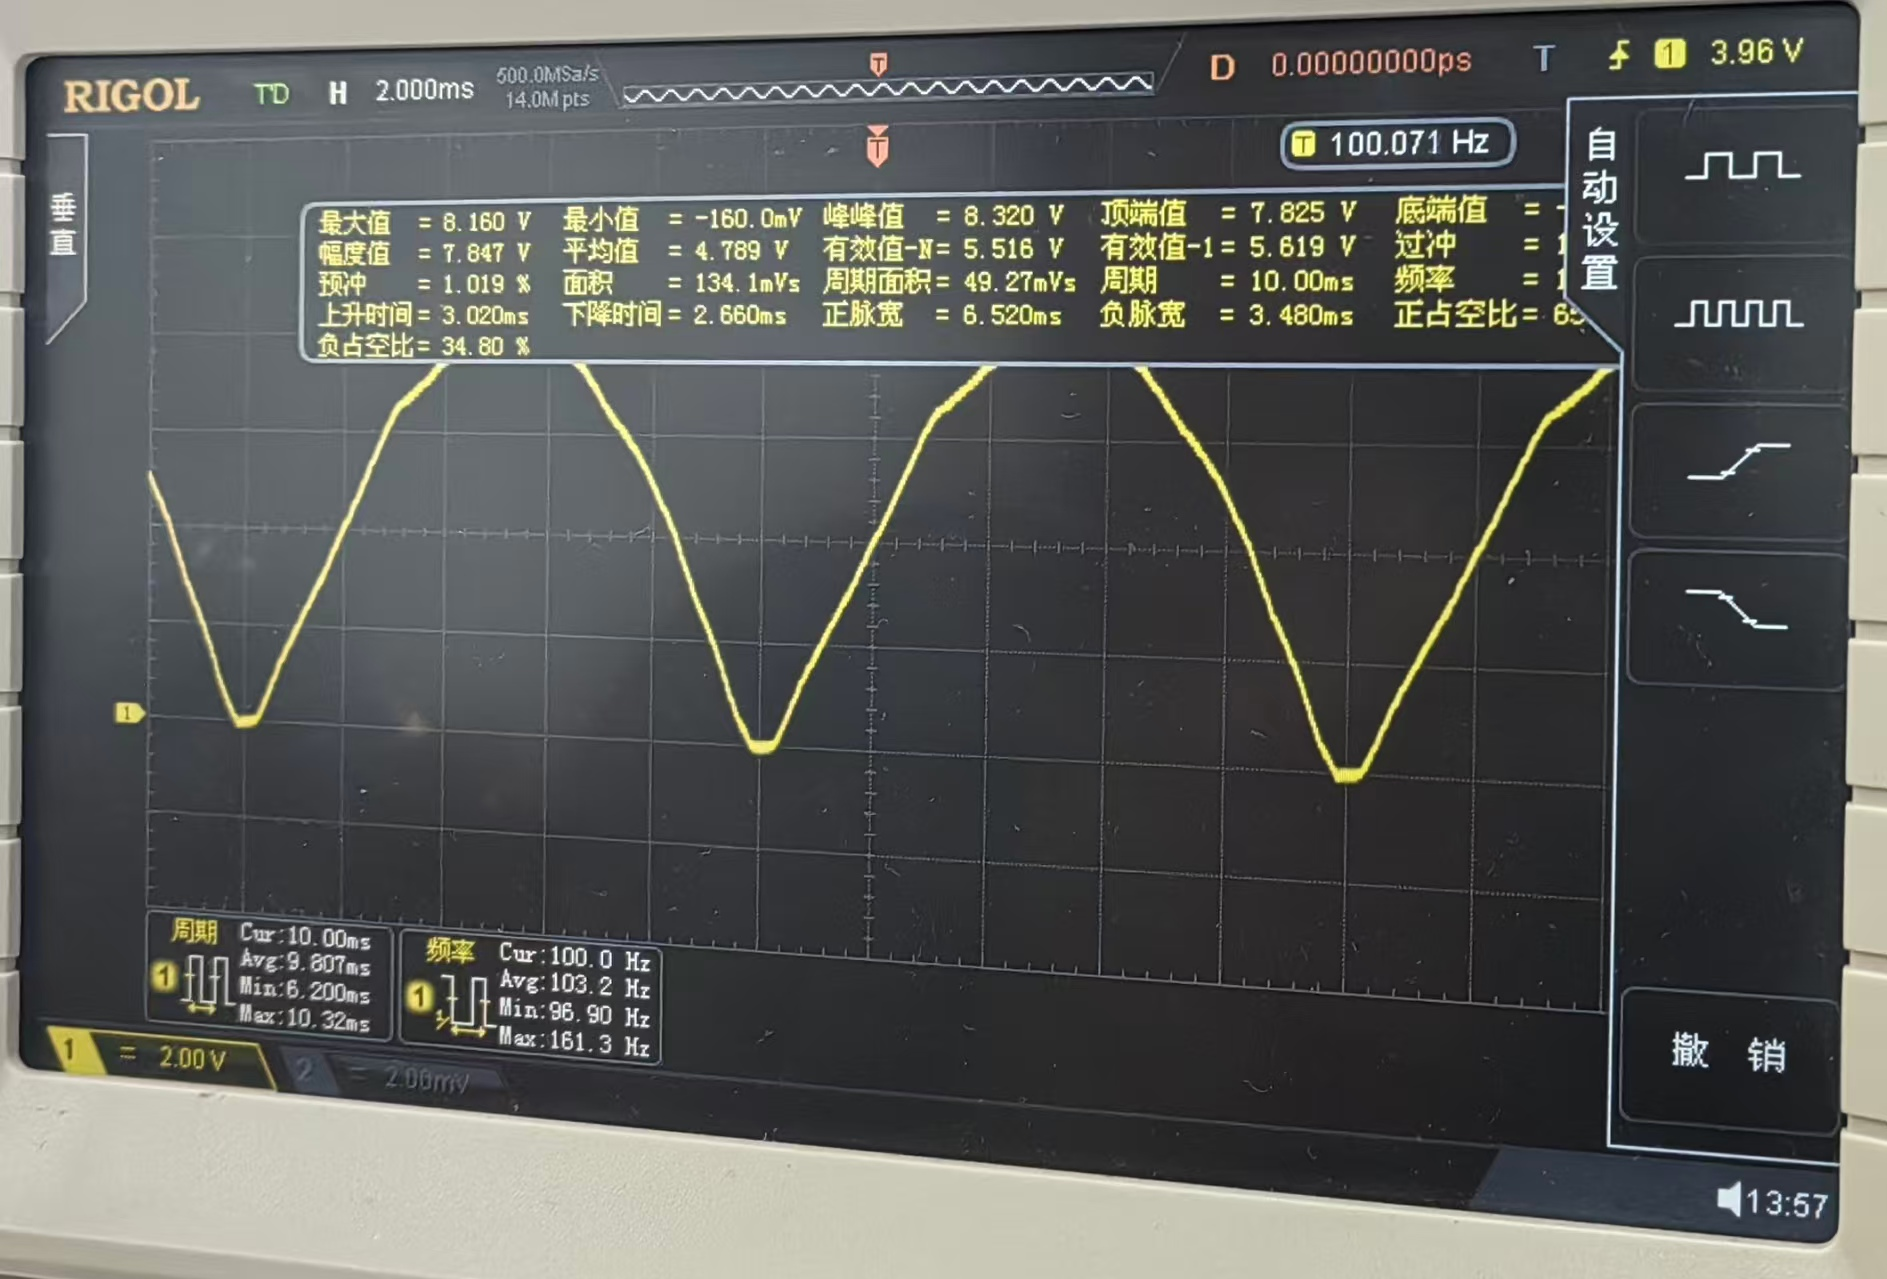
\includegraphics[width=3cm]{figures/5.jpg} &4.79V & 5.52V& 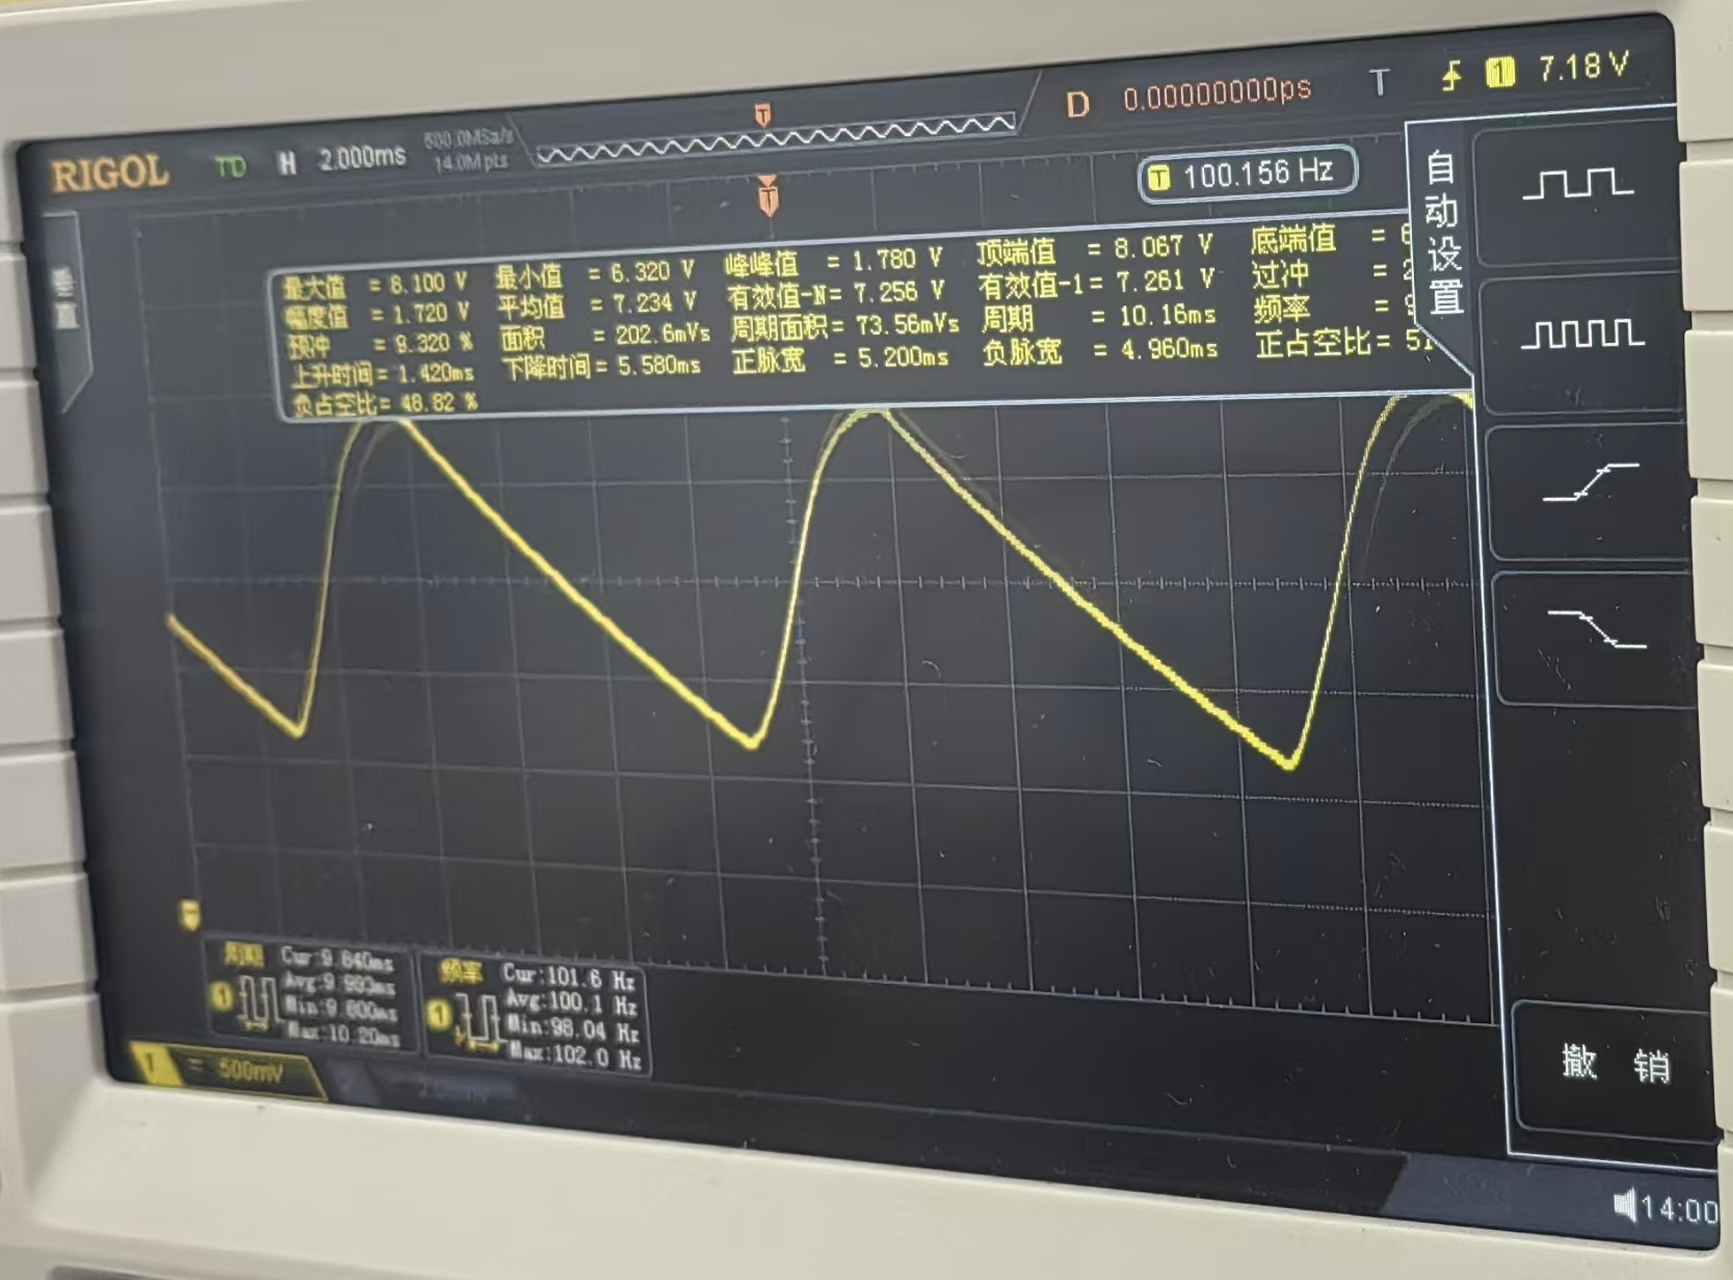
\includegraphics[width=3cm]{figures/6.jpg}\\ 
        \hline
    \end{tabular}
\end{table}

\begin{table}[H]
    \centering
    \caption{桥式整流电路}
    \vspace{0.2cm}
    % 定义6列，全部居中，带竖线
    \begin{tabular}{|c|c|c|c|c|c|}
        \hline
        % 第一行表头：合并单元格
        \multicolumn{2}{|c|}{输入信号} & 
        \multicolumn{3}{c|}{无滤波器输出信号} & 
        \makecell[c]{几十$\mu$F滤波器\\输出信号} \\
        \hline
        % 第二行表头：具体参数
        波形图 & 有效值电压 $U_2$ & 波形图 & 平均值电压 & 有效值电压 & 波形图 \\
        \hline
        % 数据行 1 (使用 vspace 增加高度，模拟空白填空区)
        \rule{0pt}{30pt} 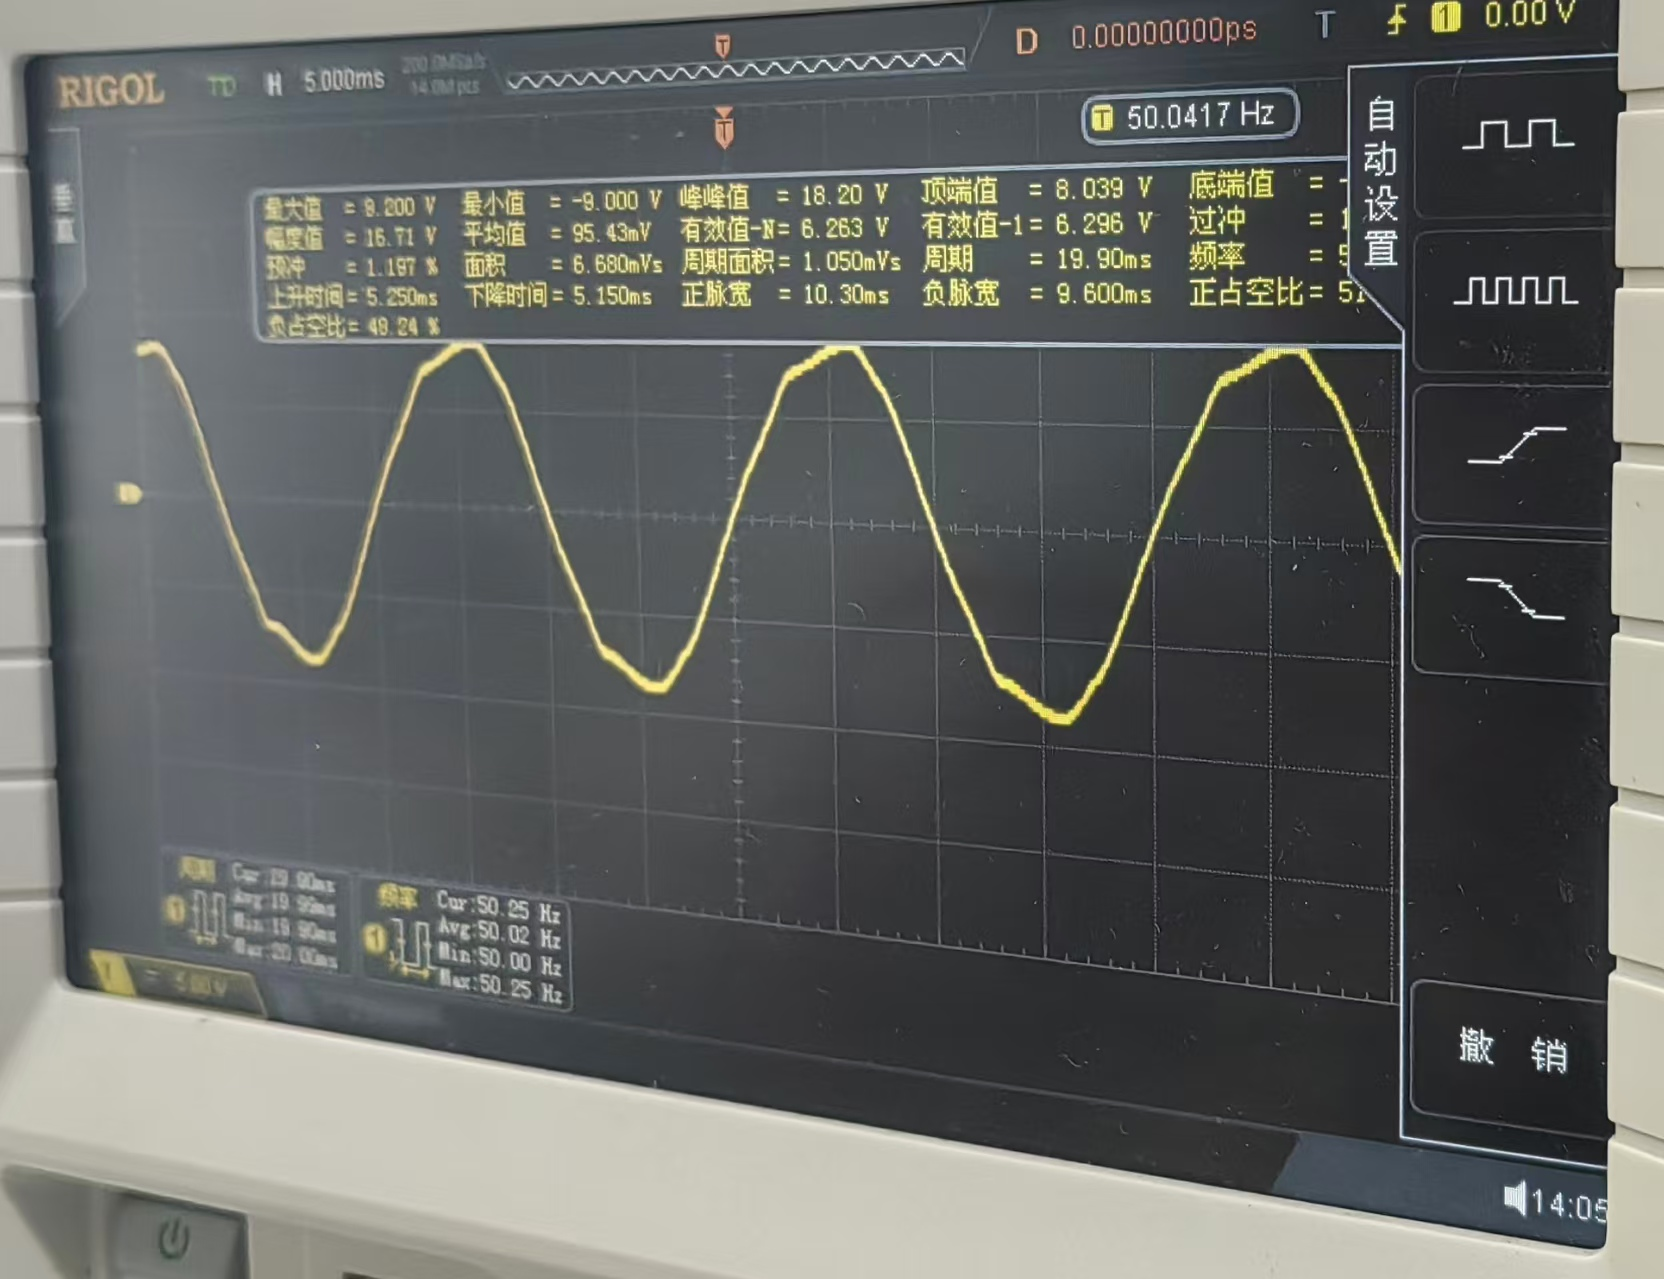
\includegraphics[width=3cm]{figures/7.jpg}& 6.30V&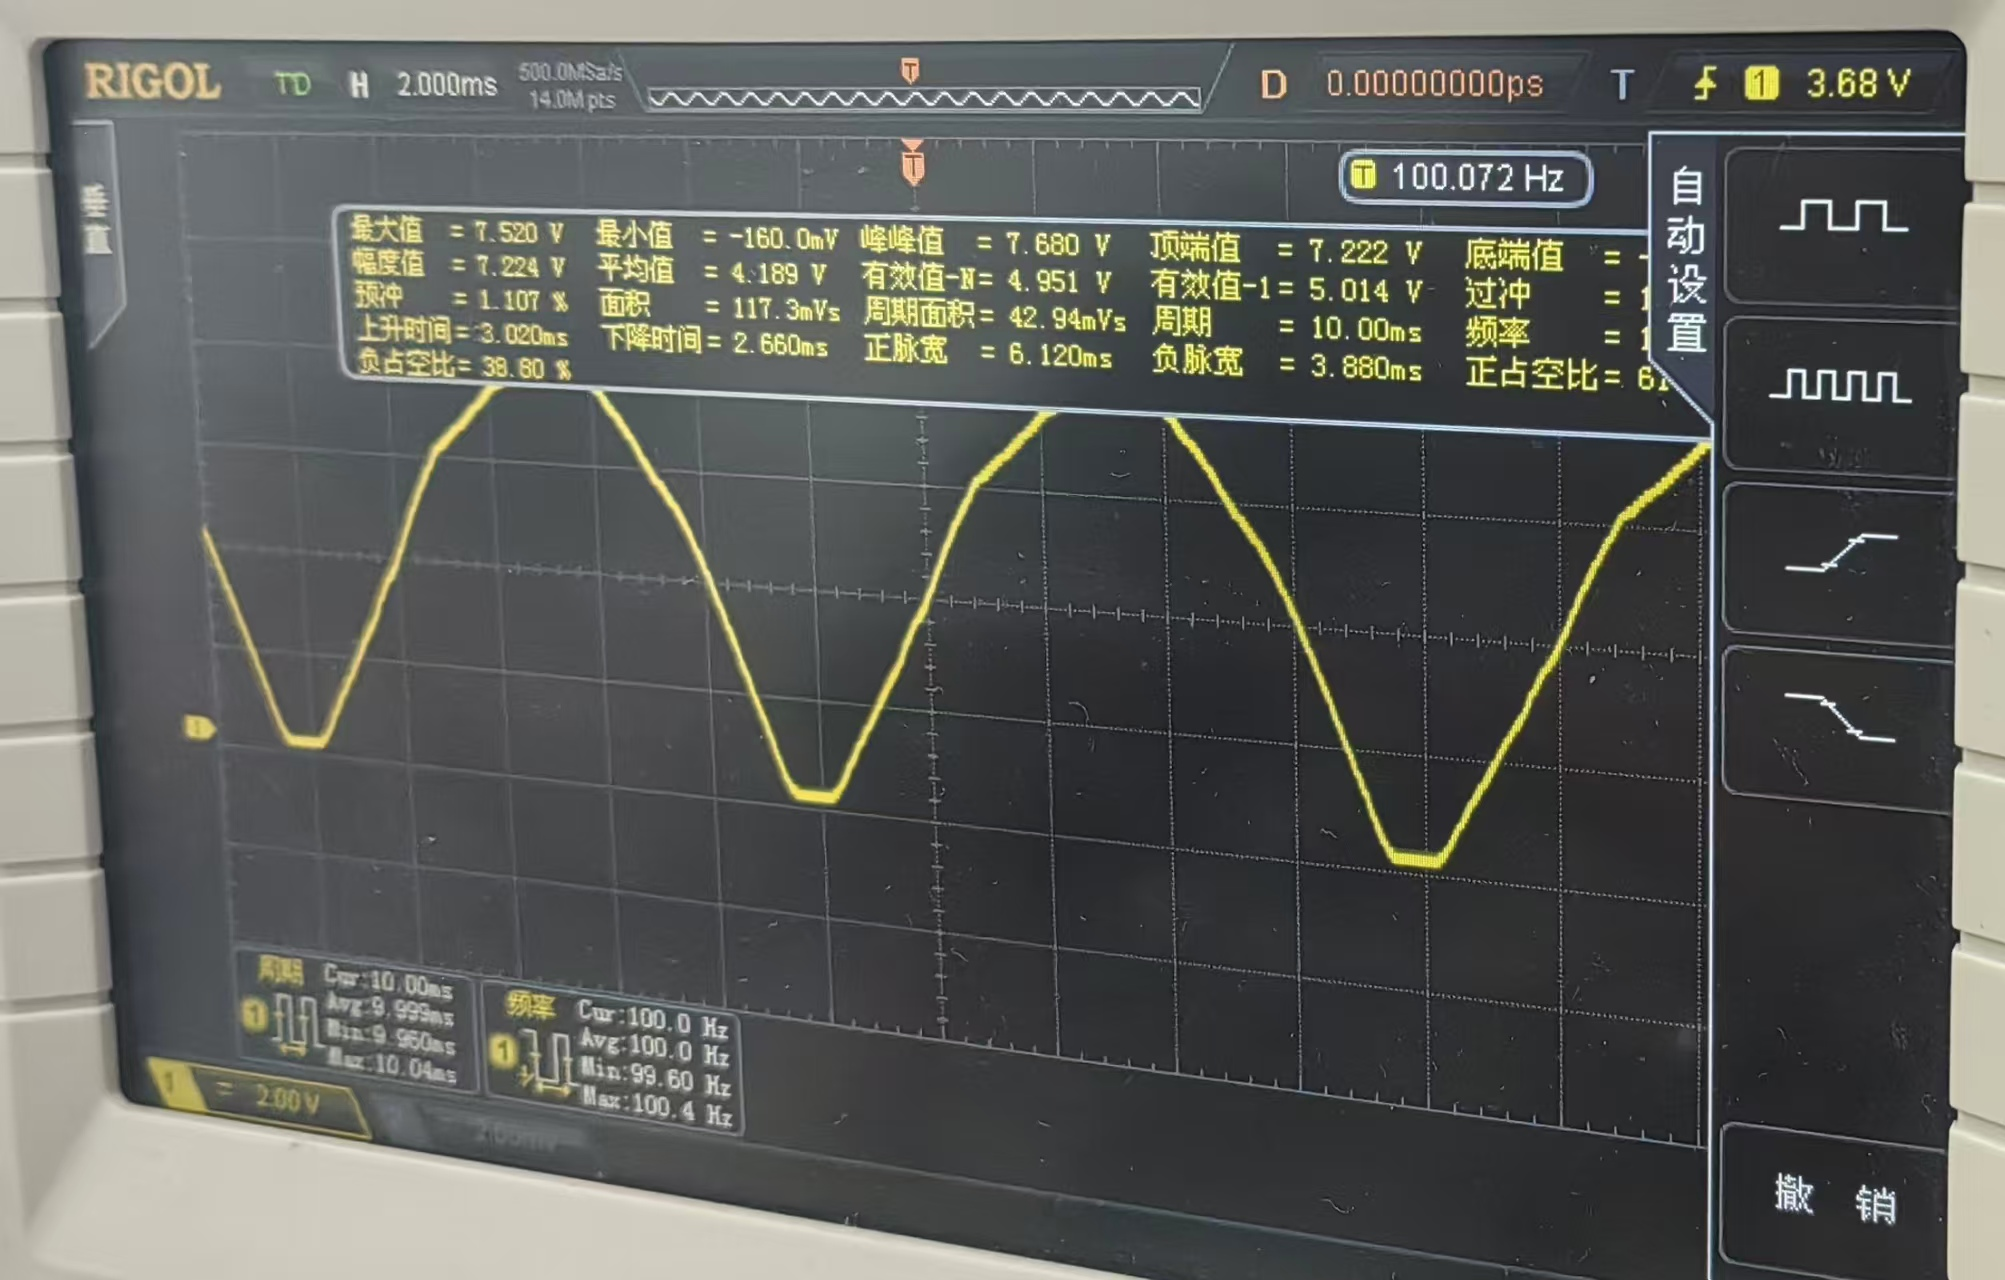
\includegraphics[width=3cm]{figures/8.jpg} &4.19V & 4.95V& 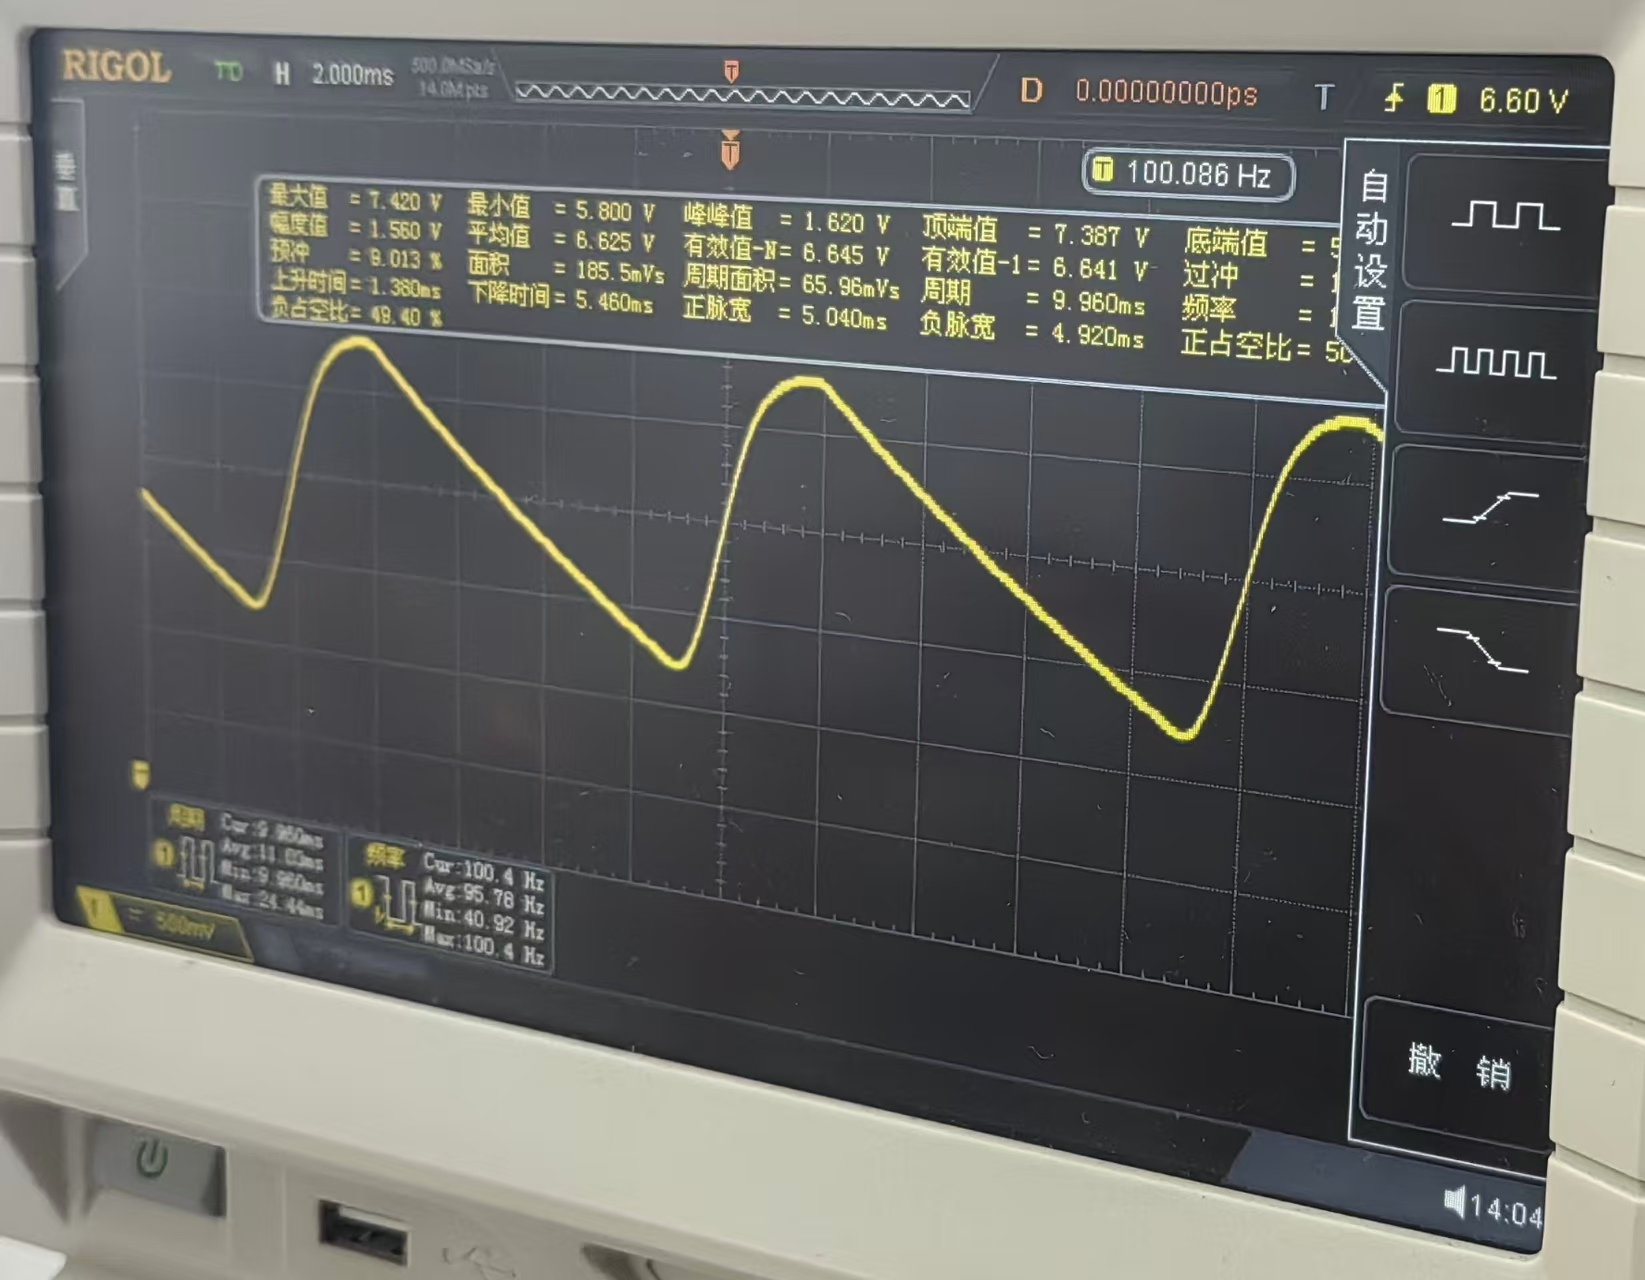
\includegraphics[width=3cm]{figures/9.jpg}\\ 
        \hline
    \end{tabular}
\end{table}

    \subsection{误差分析}
    \xiaosi （运用测量误差、相对误差、不确定度等分析实验结果，20分）

    \myspace{1}

    \textbf{交流电路功率因数实验：}
    \begin{enumerate}
        \item 电流标示数不断改变，无法稳定在一个固定值，读数是产生较大误差；
        \item 设备老化，电容实际值与标称值有偏差，接触点的电阻等对实验结果产生影响；
        \item 灯管产生大量热量，导致电阻改变，影响实验结果。
    \end{enumerate}
    
    \textbf{组装整流器实验：}
    \begin{enumerate}
        \item 电路元件较旧，导线有时接触不良，可能会对波形有一定影响；
        \item 电路中的很多元件在实际条件下非理想，存在电阻会消耗部分电能，使负载电阻阻值与标注有差别；

        \item 输入电压并非一成不变，其会有一定波动，这可能会造成变压器的工作状态产生一定浮动；
        \item 理想二极管有单向导通性，但实际器件在加反向电压时电流并非零，加正向电压时也并非完全短路。
    \end{enumerate}
    
    \subsection{实验探讨}
    \xiaosi （对实验内容、现象和过程的小结，不超过100字，10分）

    \myspace{1}
    通过本次实验，我学习了交流电功率因数的测定及其原理，学习了几种组装整流器的方法和原理，复习了常用电子元件的相关特性和示波器的使用，进一步夯实了实验基本素养和实验操作能力。

\section{思考题}

    \xiaosi （解答教材或讲义或老师布置的思考题，10分）

    \subsubsection*{提高功率因数的意义何在？为什么并联电容可以提高功率因数？并联电容是否越大越好？}

    \begin{enumerate}
        \item 提高功率因数可以减小线路电流从而降低输电损耗，同时能更充分地利用电源设备（如变压器）的容量。
        \item 并联电容产生的超前（容性）电流能抵消感性负载需要的滞后（感性）电流，从而减小总电压与总电流之间的相位差。
        \item 不是，过大的电容会导致“过补偿”使电路变为容性，这不仅会再次降低功率因数，还可能引起线路电压异常升高。

    \end{enumerate}

    \subsubsection*{总结不同的整流电路和不同滤波电路的利弊。}
    
    \begin{enumerate}
        \item 半波整流电路：结构简单，搭建方便；缺点是二极管承受的反向电压很大，变压器效率低，输出脉动大。
        \item 全波整流电路：平均值高，脉动程度低；缺点是电路结构复杂，需变压器有中心抽头，反向电压大。
        \item 单相桥式整流电路：整流效果好，反向电压小；缺点是结构相对复杂。
        \item 电容滤波：输出电压高，滤波效果好；缺点是负载能力差，充电电流大。
        \item 电感滤波：负载能力好；缺点是输出电压低，产生的电动势可能击穿元器件。
    \end{enumerate}

    
    \subsubsection*{整流和滤波的目的是什么？}
    
    答：整流和滤波的目的是将交流变为直流，尽可能得到波形平直的直流电。整流电路将交流电变为脉动直流电，滤波电路滤除脉动直流中的交流部分。    

    \subsubsection*{如何根据需要选择合适的整流电路？}

    答：半波整流电路一般用于对电源要求不高的情况，全波整流电路用于对电源要求较高的电路，单相桥式整流电路应用较广泛。
    
\newpage

\sihao\textbf{注意事项：}
\xiaosi
\begin{enumerate}
    \item  用 PDF 格式上传“实验报告”，文件名：学生姓名+学号+实验名称+周次。
    \item  “实验报告”必须递交在“学在浙大”的本课程的对应实验项目的“作业”模块内。
    \item  “实验报告”成绩必须在“浙江大学物理实验教学中心网站”-“选课系统”内查询。
    \item 教学评价必须在“浙江大学物理实验教学中心网站”-“选课系统”内进行，学生必须进行教学评价，才能看到实验报告成绩，教学评价必须在本次实验结束后 3 天内进行。
\end{enumerate}

\vspace{1cm}
\xiaosi\centering \textbf{浙江大学物理实验教学中心制}

\end{document}